%!TEX root = thesis.tex
\chapter{Tensor Network Theory} 
This section begins from a fundamental question: How to draw a tensor network diagram? In tensor network theory \cite{jordan_studies_2011} \cite{Orus2014117} \cite{bauer_tensor_2011}, we are used to represent tensors as the notations, shown in Fig.~\ref{fig211}, because \textit{tensor diagrams} can fully describe the quantum states of any geometric lattice systems explicitly. Furthermore, base on its clear representation, the implementation of tensor network algorithms become simply. 

\section{Representation of tensors in tensor Networks}
\label{notations}
In mathematical concept, a tensor is considered as a multi-dimensional array of scalers. The arrangement of the elements in a tensor is dependent on its \textit{indices} and the \textit{rank} of a tensor, where the rank of a tensor is equivalent to the number of indices. Thus, a scaler $T$, a vector $T_{i}$ and a matrix $T_{ij}$ can be recognized as a rank-0, rank-1 and rank-2 tensor, and so on. 

Graphically, we usually use a node and few bonds to represent a tensor. Some specified examples are shown in Fig.~\ref{fig211}, the number of bond is equal to the rank of a tensor. For example, the notations without bonds, with a single bond, with two bonds and with $N$ bonds are considered as scalers, vectors, matrices and rank$N$ tensors. Moreover, the dimension of a rank-$N$ tensor, $D_{total}$, is dependent on the dimensions of the bonds except that the dimension of a rank-0 tensor (scaler) is 1,
\begin{align}
	D_{total} = \begin{cases}
		1 & \text{, if $N = 0$} \\
		\chi_{1}\chi_{2}\chi_{3} \dots \chi_{N} & \text{, if $N \neq 0$}
	\end{cases}
\end{align}
For instance, assume that the dimensions of the bonds of the rank-3 tensor $T_{\alpha \beta \gamma}$, shown in Fig.~\ref{fig211}(iv) are $\chi_{\alpha}$, $\chi_{\beta}$ and $\chi_{\gamma}$. The tensor $T_{\alpha \beta \gamma}$ contains $\chi_{\alpha}$$\chi_{\beta}$$\chi_{\gamma}$ components.

\begin{figure}[ht]
	\centering
	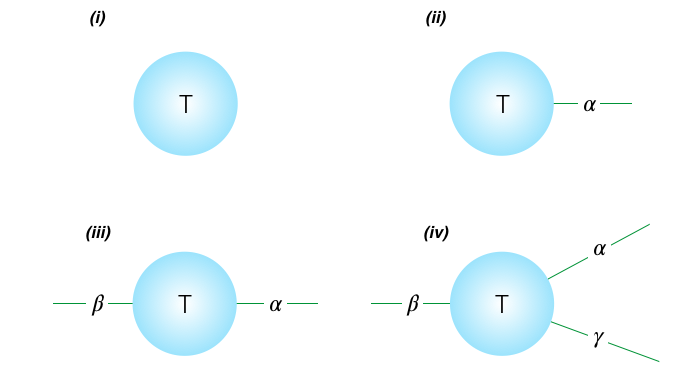
\includegraphics[width=0.80\textwidth]{figures/fig211.png}
	\caption[The reprecentation of commen tensors.]{(i) A tensor without bonds is a scaler $T$, (ii) A tensor with one bond is a vector $T_{\alpha}$, (iii) A tensor with two bonds is a Matrix $T_{\alpha \beta}$, (iv) A tensor with three bonds is a rank-3 tensor $T_{\alpha \beta \gamma}$.}
	\label{fig211}
\end{figure}

\section{Tensor operations and tensor network diagrams} % (fold)
\label{operation}
In the computational languages, a fold tensor can be regard as a container of the elements. It is not endowed with meanings until unfolded to a specified shape. In other words, we must transform it to a tensor less than rank-3 before doing operations. The process is also called \textit{permuteation}.

\subsection{Permutation}
See Fig.~\ref{fig224}, the goal of this example is to the permute the tensor $A_{\alpha \beta \gamma}$ into $\hat{A}_{\alpha \gamma \beta}$,
\begin{figure}[ht]
	\centering
	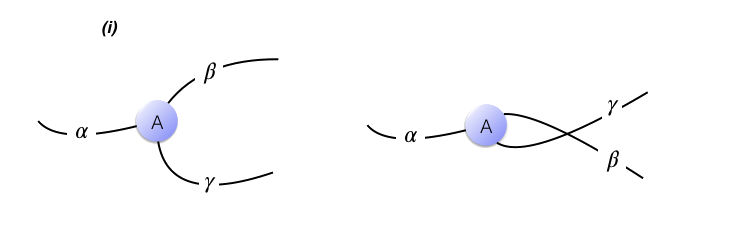
\includegraphics[width=0.80\textwidth]{figures/fig224.png}
	\caption[The permutation of a tensor.]{ Permute tensor $A_{\alpha \beta \gamma}$ to $\hat{A}_{\alpha \gamma \beta}$ }
	\label{fig224}
\end{figure}
\begin{align}
	A_{\alpha \beta \gamma} \rightarrow \hat{A}_{\alpha \gamma \beta}
\end{align}
Nevertheless, the arrangements of tensor $A_{\alpha \beta \gamma}$ is modified to $\hat{A}_{\alpha \gamma \beta}$. The components of them are exact equivalence. 

\begin{figure}[ht]
	\centering
	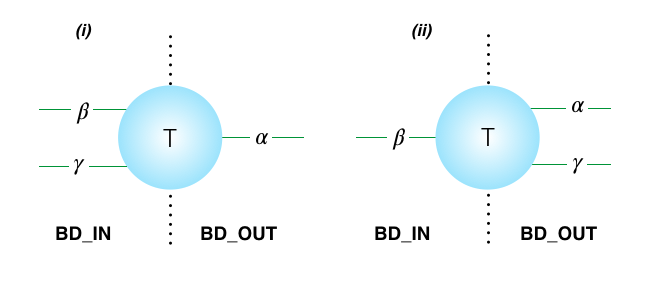
\includegraphics[width=0.80\textwidth]{figures/fig221.png}
	\caption[Representaion of unfold tensors.]{(i) Unfold a tensor to a matrix $T_{\chi_{\beta}\chi_{\gamma},\chi_{\alpha}}$, (ii) Unfold a tensor to a matrix $T_{\chi_{\beta},\chi_{\alpha}\chi_{\gamma}}$.}
	\label{fig221}
\end{figure}

In order to explain more clearly, we separate the tensor to two part, incoming (BD\_IN) and outgoing (BD\_OUT) which are also designed for distinguishing different types of \textit{uni10::Bond} in \textit{Uni10 Library} \cite{}, to show what the meaning of reshape is in the linear algebra. The total dimensions of the bonds in the part BD\_IN and BD\_OUT corresponds to the number of rows and columns of a matrix. For instance, if the indices of $T_{\alpha \beta \gamma}$ ordered like Fig.~\ref{fig221}(i), $T_{\alpha \beta \gamma}$ is equivalent to a matrix $M_{\chi_{\beta}\chi_{\gamma},\chi_{\alpha}}$, where $\chi_{\alpha}$, $\chi_{\beta}$ and $\chi_{\gamma}$ are the dimensions of the bonds, $\alpha$, $\beta$ and $\gamma$. Similarity, The tensor shown as Fig.~\ref{fig221}(ii) can be recognized as a matrix $M_{\chi_{\beta},\chi_{\alpha}\chi_{\gamma}}$.

\subsection{Tensor contraction}
Tensor contraction is defined as the sum of all products of the shared indices of tensors. For instance, the tensor diagram of contracting two rank-2 tensors $A_{\alpha \beta}$ and $B_{\beta \gamma}$ is shown as Fig.~\ref{fig222}(i) which can be written as, 
\begin{align}
	C_{\alpha \gamma}=\sum\limits_{\beta = 1}^{\chi_{\beta}}{A_{\alpha \beta}B_{\beta \gamma}},
\end{align}
and obviously this example corresponds to the inner-product of two matrices $A_{\chi_{\alpha}, \chi{\beta}}$ and $B_{\chi_{\beta}, \chi_{\gamma}}$,
\begin{figure}[ht]
	\centering
	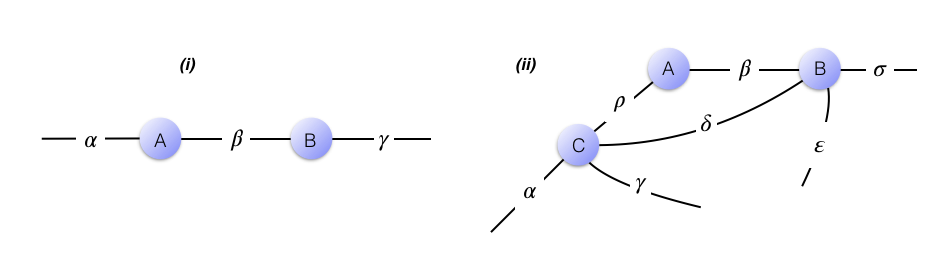
\includegraphics[width=0.80\textwidth]{figures/fig222.png}
	\caption[The examples of tensor diagrams.]{(i) Contract rank-2 tensors $A_{\alpha \beta}$ and $B_{\beta \gamma} $ (ii) Contract a rank-2 tensor $A_{\rho \beta}$, and two rank-4 tensors $B_{\sigma \varepsilon \delta}$ and $C_{\delta \rho \alpha}$}
	\label{fig222}
\end{figure}

Now that we considered a more complicated example, see Fig\ref{fig222}(ii). The equation of the tensor diagram is described as,
\begin{align}
	D_{\alpha \gamma \sigma \epsilon}=\sum_{\beta \rho \delta}{A_{\rho \beta}B_{\beta \sigma \epsilon \delta}C_{\gamma \delta \rho \alpha}},
\end{align}

In order to contract the tensors $A_{\rho \beta}$, $B_{\beta \sigma \epsilon \delta}$ and $C_{\gamma \delta \rho \alpha}$ in the diagram, we can follow the contraction processes in Fig.~\ref{fig223}
\begin{enumerate}
	\item Select a pair of tensors arbitrarily: In the example, we choose the tensor $A_{\rho \beta}$ and $C_{\gamma \alpha \delta \rho}$ at first. 
	\item Permute the tensors to specific shape and operate the inner-product: As shown in Fig.~\ref{fig223}(ii)-(iii) Reshape (unfold) $A_{\rho \beta}$ and $C_{\gamma \alpha \delta}$ to matrices $A_{\chi_{\rho}, \chi_{\beta}}$ and $C_{\chi_{\gamma} \chi_{\alpha} \chi_{\delta} \chi_{\rho}}$ and inner product two matrices, 
		\begin{align}
			\theta_{\gamma \alpha \delta \beta} = C_{\chi_{\gamma} \chi_{\alpha} \chi_{\delta} \chi_{\rho}} \cdot A_{\chi_{\rho}, \chi_{\beta}}
		\end{align}
	\item Repeat the step (1) and (2) until all tensors are contracted: See Fig.~\ref{fig223}(iii)-(iv), repeat the steps again to contract the remained tensors $\theta_{\gamma \alpha \delta \beta}$ and $B_{\beta \sigma \delta \varepsilon}$
\end{enumerate}

\begin{figure}[ht]
	\centering
	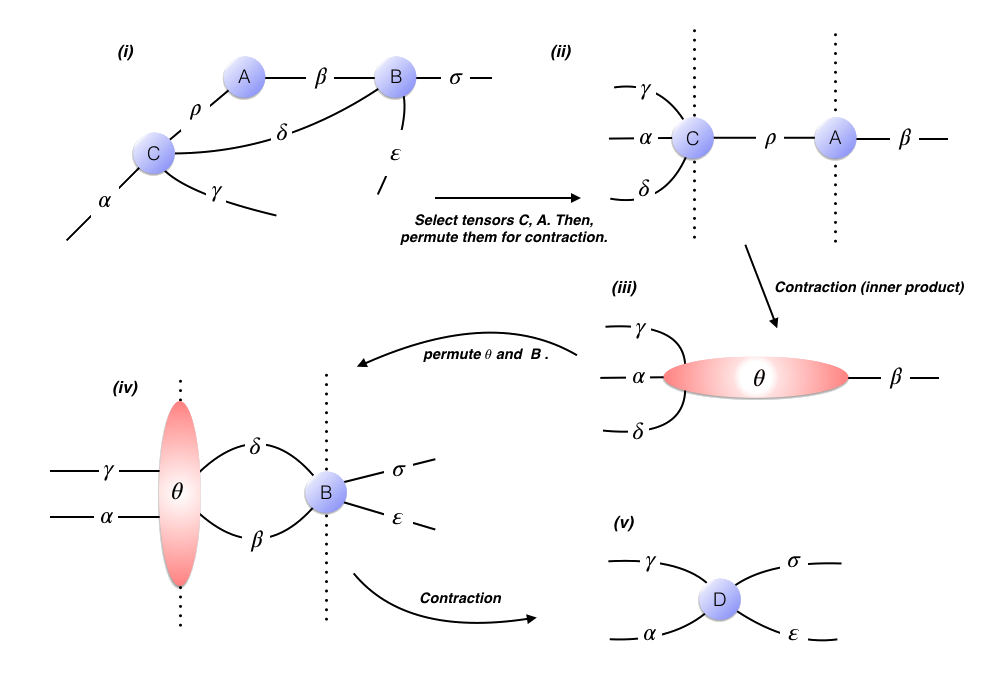
\includegraphics[width=0.95\textwidth]{figures/fig223.png}
	\caption[The contraction procedures of the network shown in Fig\ref{fig222}(ii)]{ The contraction procedures of the network shown in Fig\ref{fig222}}
	\label{fig223}
\end{figure}

Actually, the choice in step (1) is restricted in some algorithms, such as corner transfer matrix \cite{PhysRevB.85.205117} and fast full update \cite{PhysRevB.92.035142}, because the order of the contraction network is strongly correlated to the efficiency. For example, if the dimensions of the bonds of the tensors, $A_{\rho \beta}$, $B_{\beta \sigma \epsilon \delta}$ and $C_{\gamma \delta \rho \alpha}$ in Fig.~\ref{fig223}(i), are $D$. The consumption of the contraction of $A_{\rho \beta}$ and $C_{\gamma \delta \rho \alpha}$ is $D^4$. However, if we contract $B_{\beta \sigma \epsilon \delta}$ and $C_{\gamma \delta \rho \alpha}$ at first, it will increase to $D^6$. Therefor, how to determine the cheapest contraction order is a significant issue \cite{PhysRevE.90.033315}.

\section{Describe Quantum states with tensor network} % (fold)
\label{sub:map2quan}
Before drawing a many-body system with tensor-network representation, we should discuss how to describe a spin chain composed by $N$ particles, with each particles having $d$ states. The system can be regard as a congregation of $N$ localized particles and we have recognized that a pure state corresponds to a vector in Hilbert space. Hence, the wave-function of many-body systems can be described by $N$ subspace,
\begin{align}
	\Ket{\Psi_{N}} =\sum_{i_1,i_2,\ldots,i_N}{C_{i_1,i_2,i_3,\ldots,i_N}\Ket{i_1}\otimes\Ket{i_2}\otimes \ldots \otimes \Ket{i_N}},
	\label{wavefunc}
\end{align}
where each individual $\Ket{i_1}, \Ket{i_2},\ldots, \Ket{i_N}$ spanned by an orthogonal basis , with the degree of freedom $d$. After writing down the formulation of the wave-function, Eq.~\ref{wavefunc}, we are able to build a tensor-network representation for quantum states. The wave-function $\Ket{\Psi_N}$ is shown as Fig.~\ref{fig225}(a), each bond of the tensor corresponds to the local Hilbert space $\Ket{i_n}$ and the dimension of it is equivalent to the probable states of the particle on the $n$-th site and the coefficients of the rank-N tensor corresponds to $C_{i_1,i_2,i_3,\ldots,i_N}$.

No matter from Eq.~\ref{wavefunc} or Fig.~\ref{fig225}(a), we can notice that the number of coefficients in $C_{i_1,i_2,i_3,\ldots,\i_N}$ is proportional to $d^N$, directly. Therefor, it is impossible to fully describe a many-body system by a classical machine if the system size larger then fifty. Fortunately, according to the theory of MPS \cite{PhysRevB.73.094423} \cite{PhysRevLett.75.3537}, the wave-function can be decomposed to two subsystem by Schmidt decomposition and there are more discussions in the Chap.\ref{chapter:2ditebd}. 
\begin{figure}[ht]
	\centering
	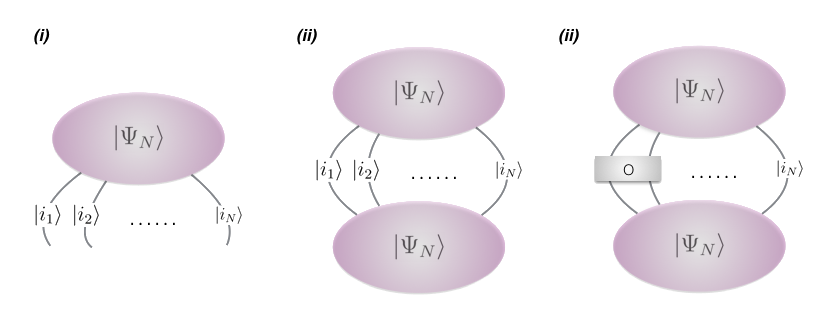
\includegraphics[width=0.85\textwidth]{figures/fig225.png}
	\caption[Represent wave-function of quntum states of TN]{(i) The wave-function, $\Ket{\Psi_N}$ (ii) The norm of $\Ket{\Psi_N}$, $\Braket{\Psi_N|\Psi_N}$ (iii) Expectation value of observable $O$, $\Bra{\Psi_N}O\Ket{\Psi_N}$}
	\label{fig225}
\end{figure}
